\section{Downstream metrics}
The evaluation of the model in terms of the loss is not quite objective for the current problem. Even when one model might have a smaller loss, it doesn't nessecarily will perform better than another model. (cite Cohen) Therefore the evaluation of the model is done in terms of the metrics that are defined as follows. The most used ones by the clients were
\begin{itemize}
    \item Number of nuclei
    \item The relatuve area of the nuclei
    \item Total intensity
    \item Mean intensity
\end{itemize}

\subsection{Nuclei segmentation}
To properly eavluate these metrics on model predictions, post-processing first for segmenting the nuclei is needed. This is not a very straight-forward task to do as there are different edge cases where the nuclei are difficult to segment due to the variety of different factors. 

For example, different brightness of the images that comes from different exposure during the photo taking process might make the nuclei segmentation more challenging. The same goes for the different lighting conditions. Different lighning conditions are presented in Figure \ref{fig:lightning_conditions}. The following inconsistenties in lightning conditions are presented (from left to right): image contains too few cells, which leads to background being much darker than usually; overexposure of one cell, which leads to difficulties of sigmenting the rest of the cells as they are hard distinguishable from the background; lighting gradient from darker (left bottom corner) to brighter (upper right corner) region; normal lighting conditions.

Another challenge for segmentation bring nuclei that are very close to each other. This might happens sometimes because some of the cells are currently in the process of the division, some have already divided, but still located close to one another.

\begin{figure}
    \centering
    \setkeys{Gin}{width=\linewidth}
    \centering
        \begin{tabularx}{\textwidth}{YYYY}
            \textbf{Too few cells} &
            \textbf{Overexposure} &
            \textbf{Light gradient} &
            \textbf{Normal lightning} \\
            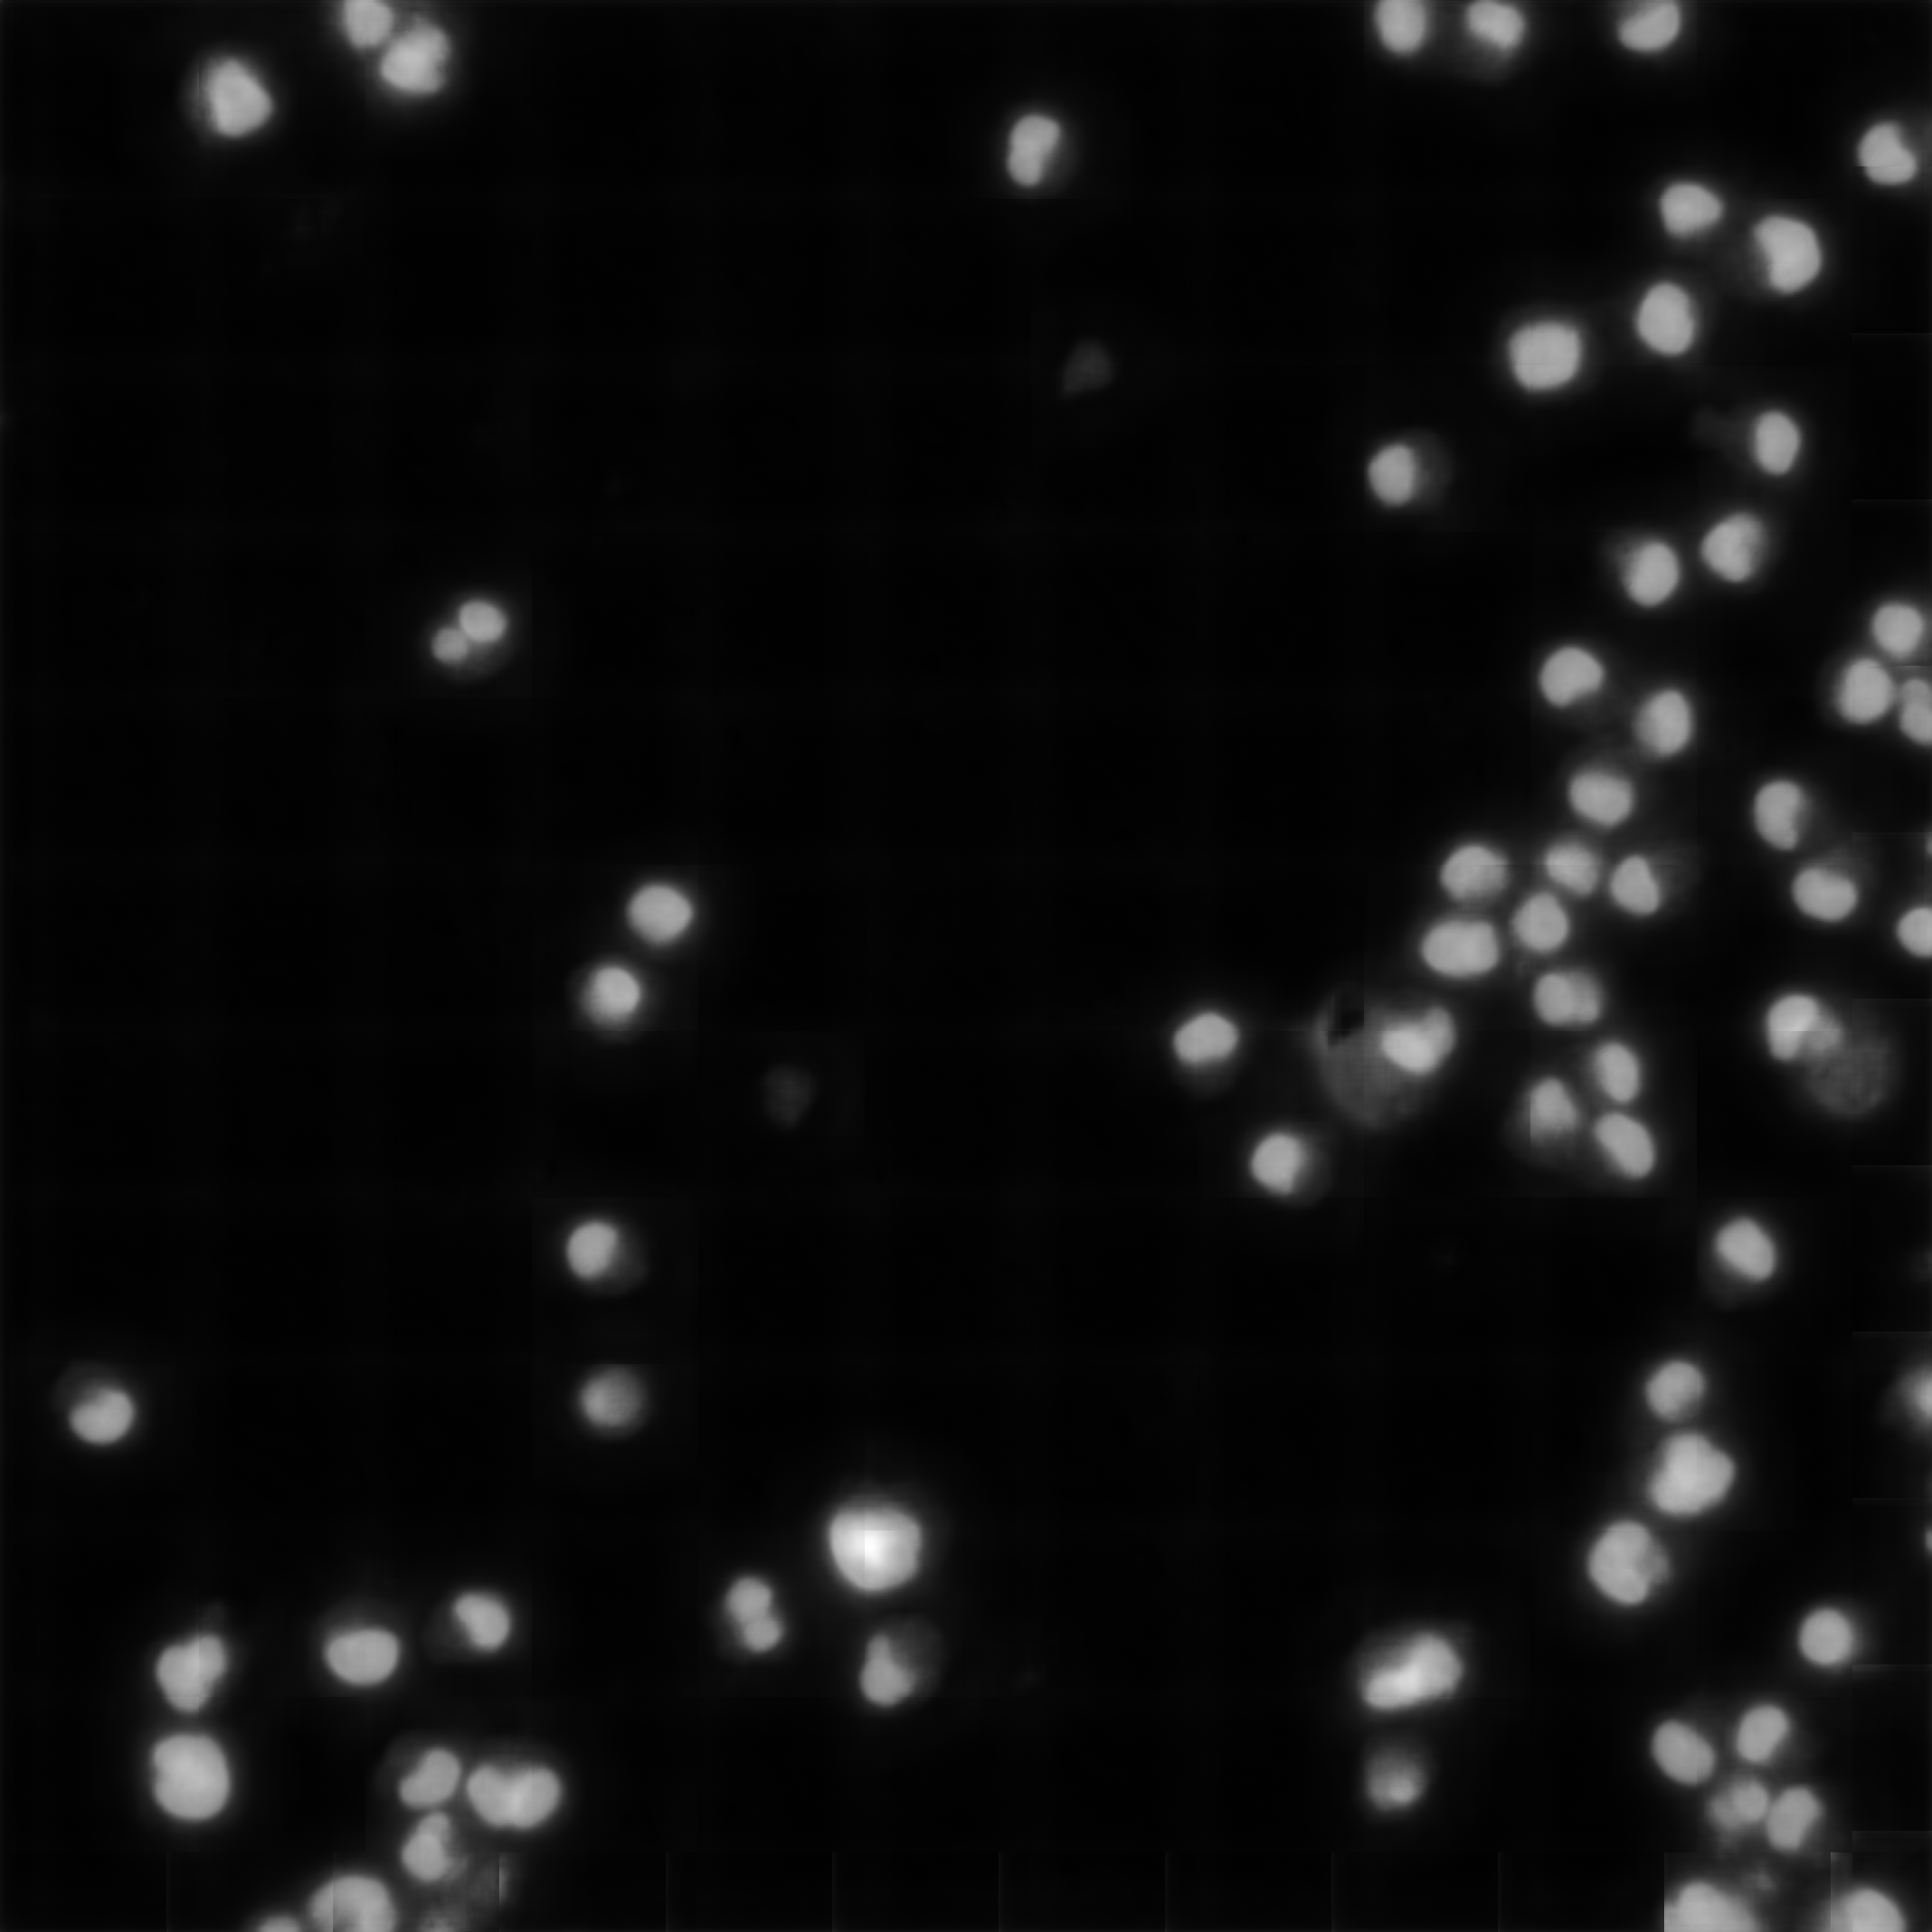
\includegraphics{bilder/lightning-conditions/lightning-1.png} & 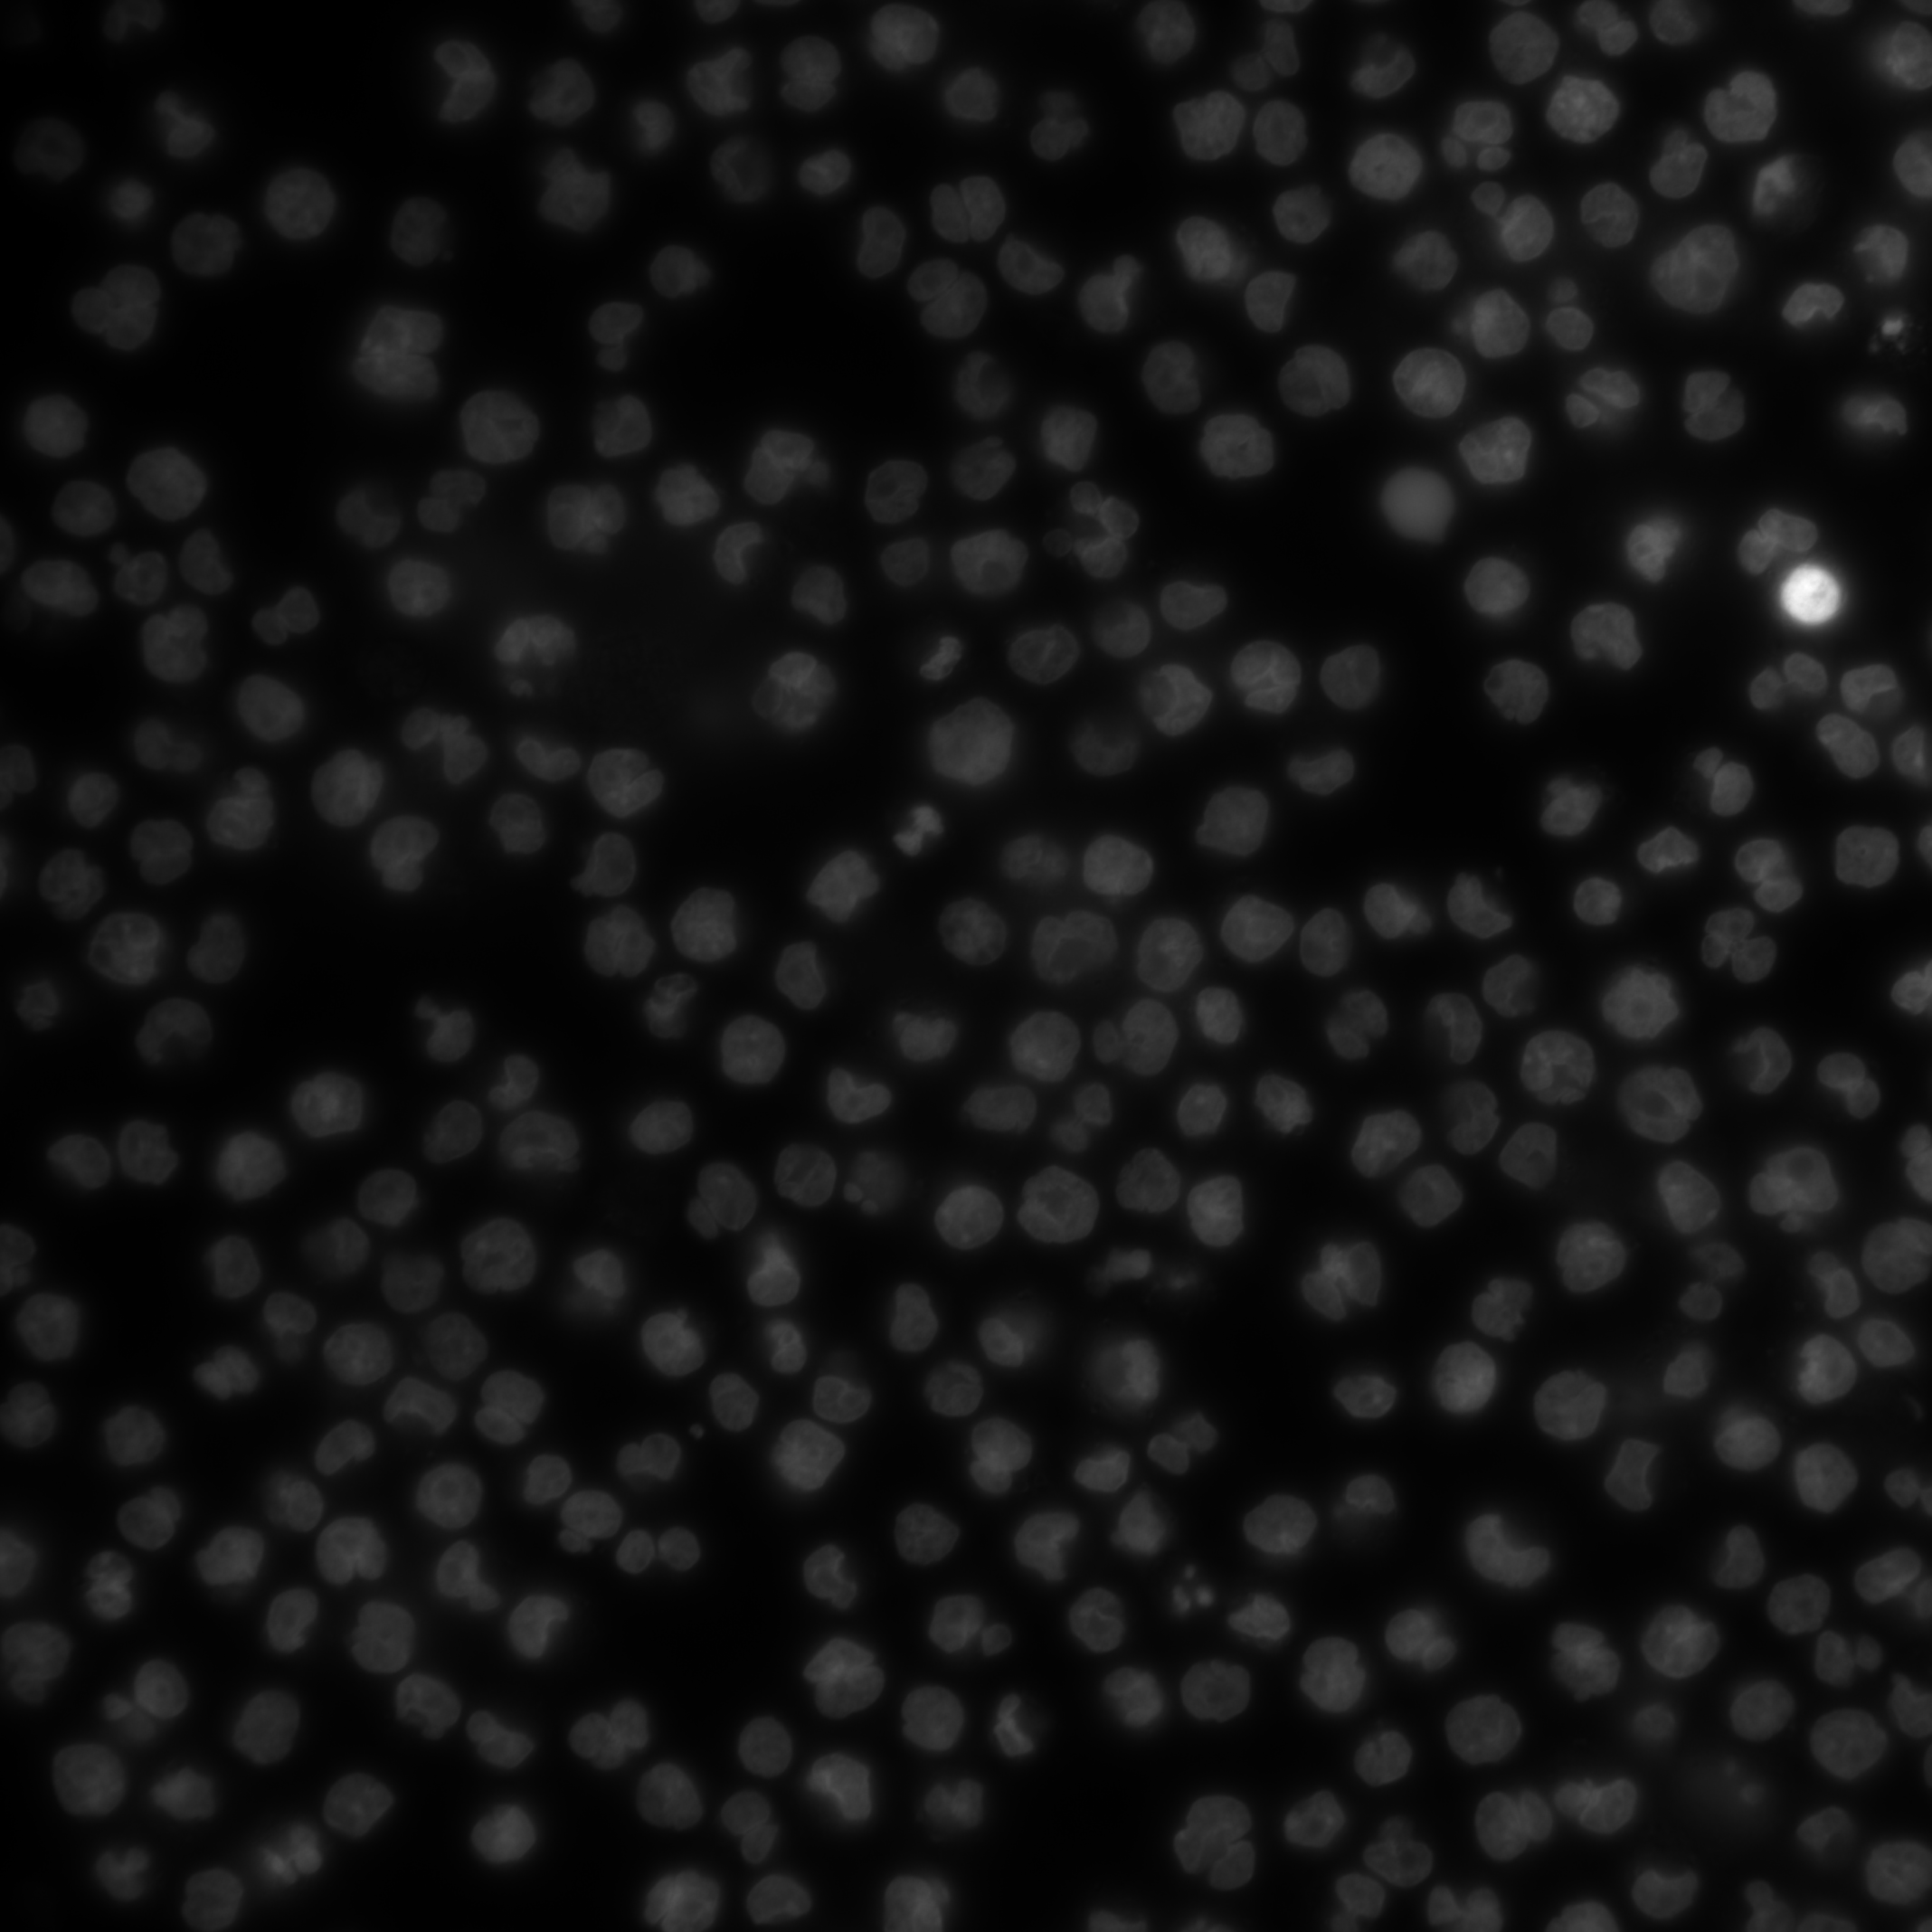
\includegraphics{bilder/lightning-conditions/lightning-2.png} &
            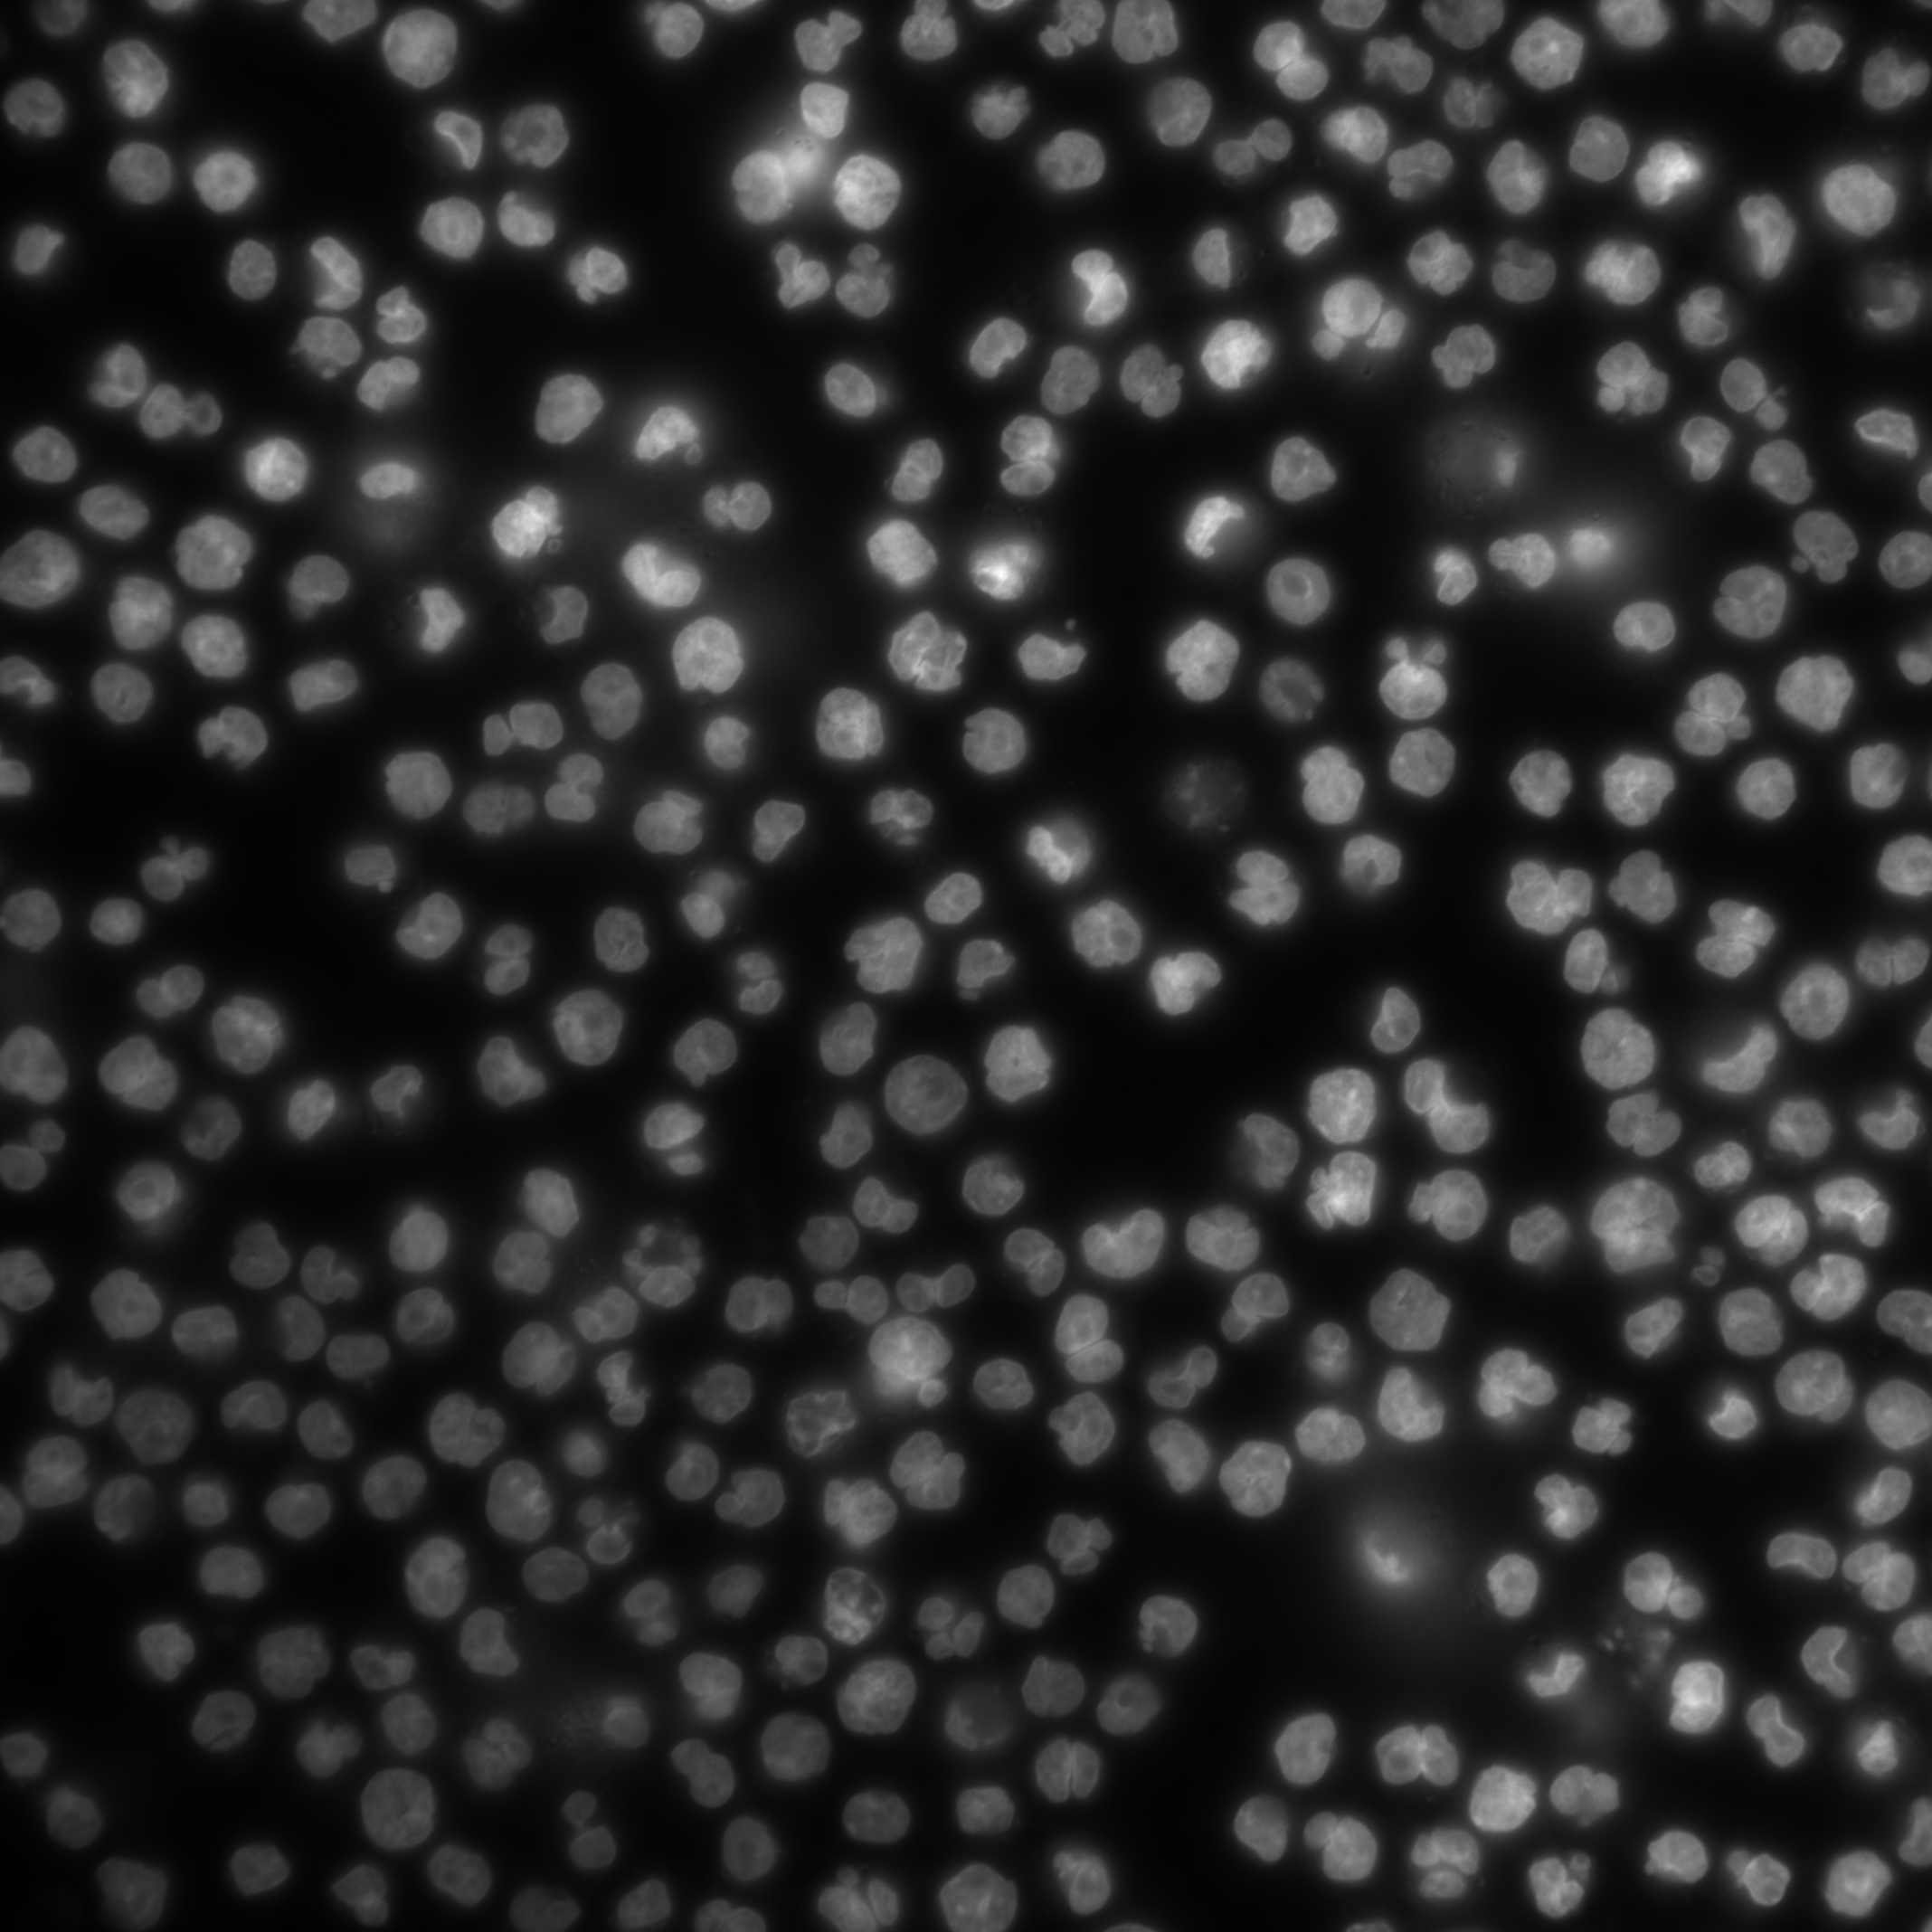
\includegraphics{bilder/lightning-conditions/lightning-3.png} & 
            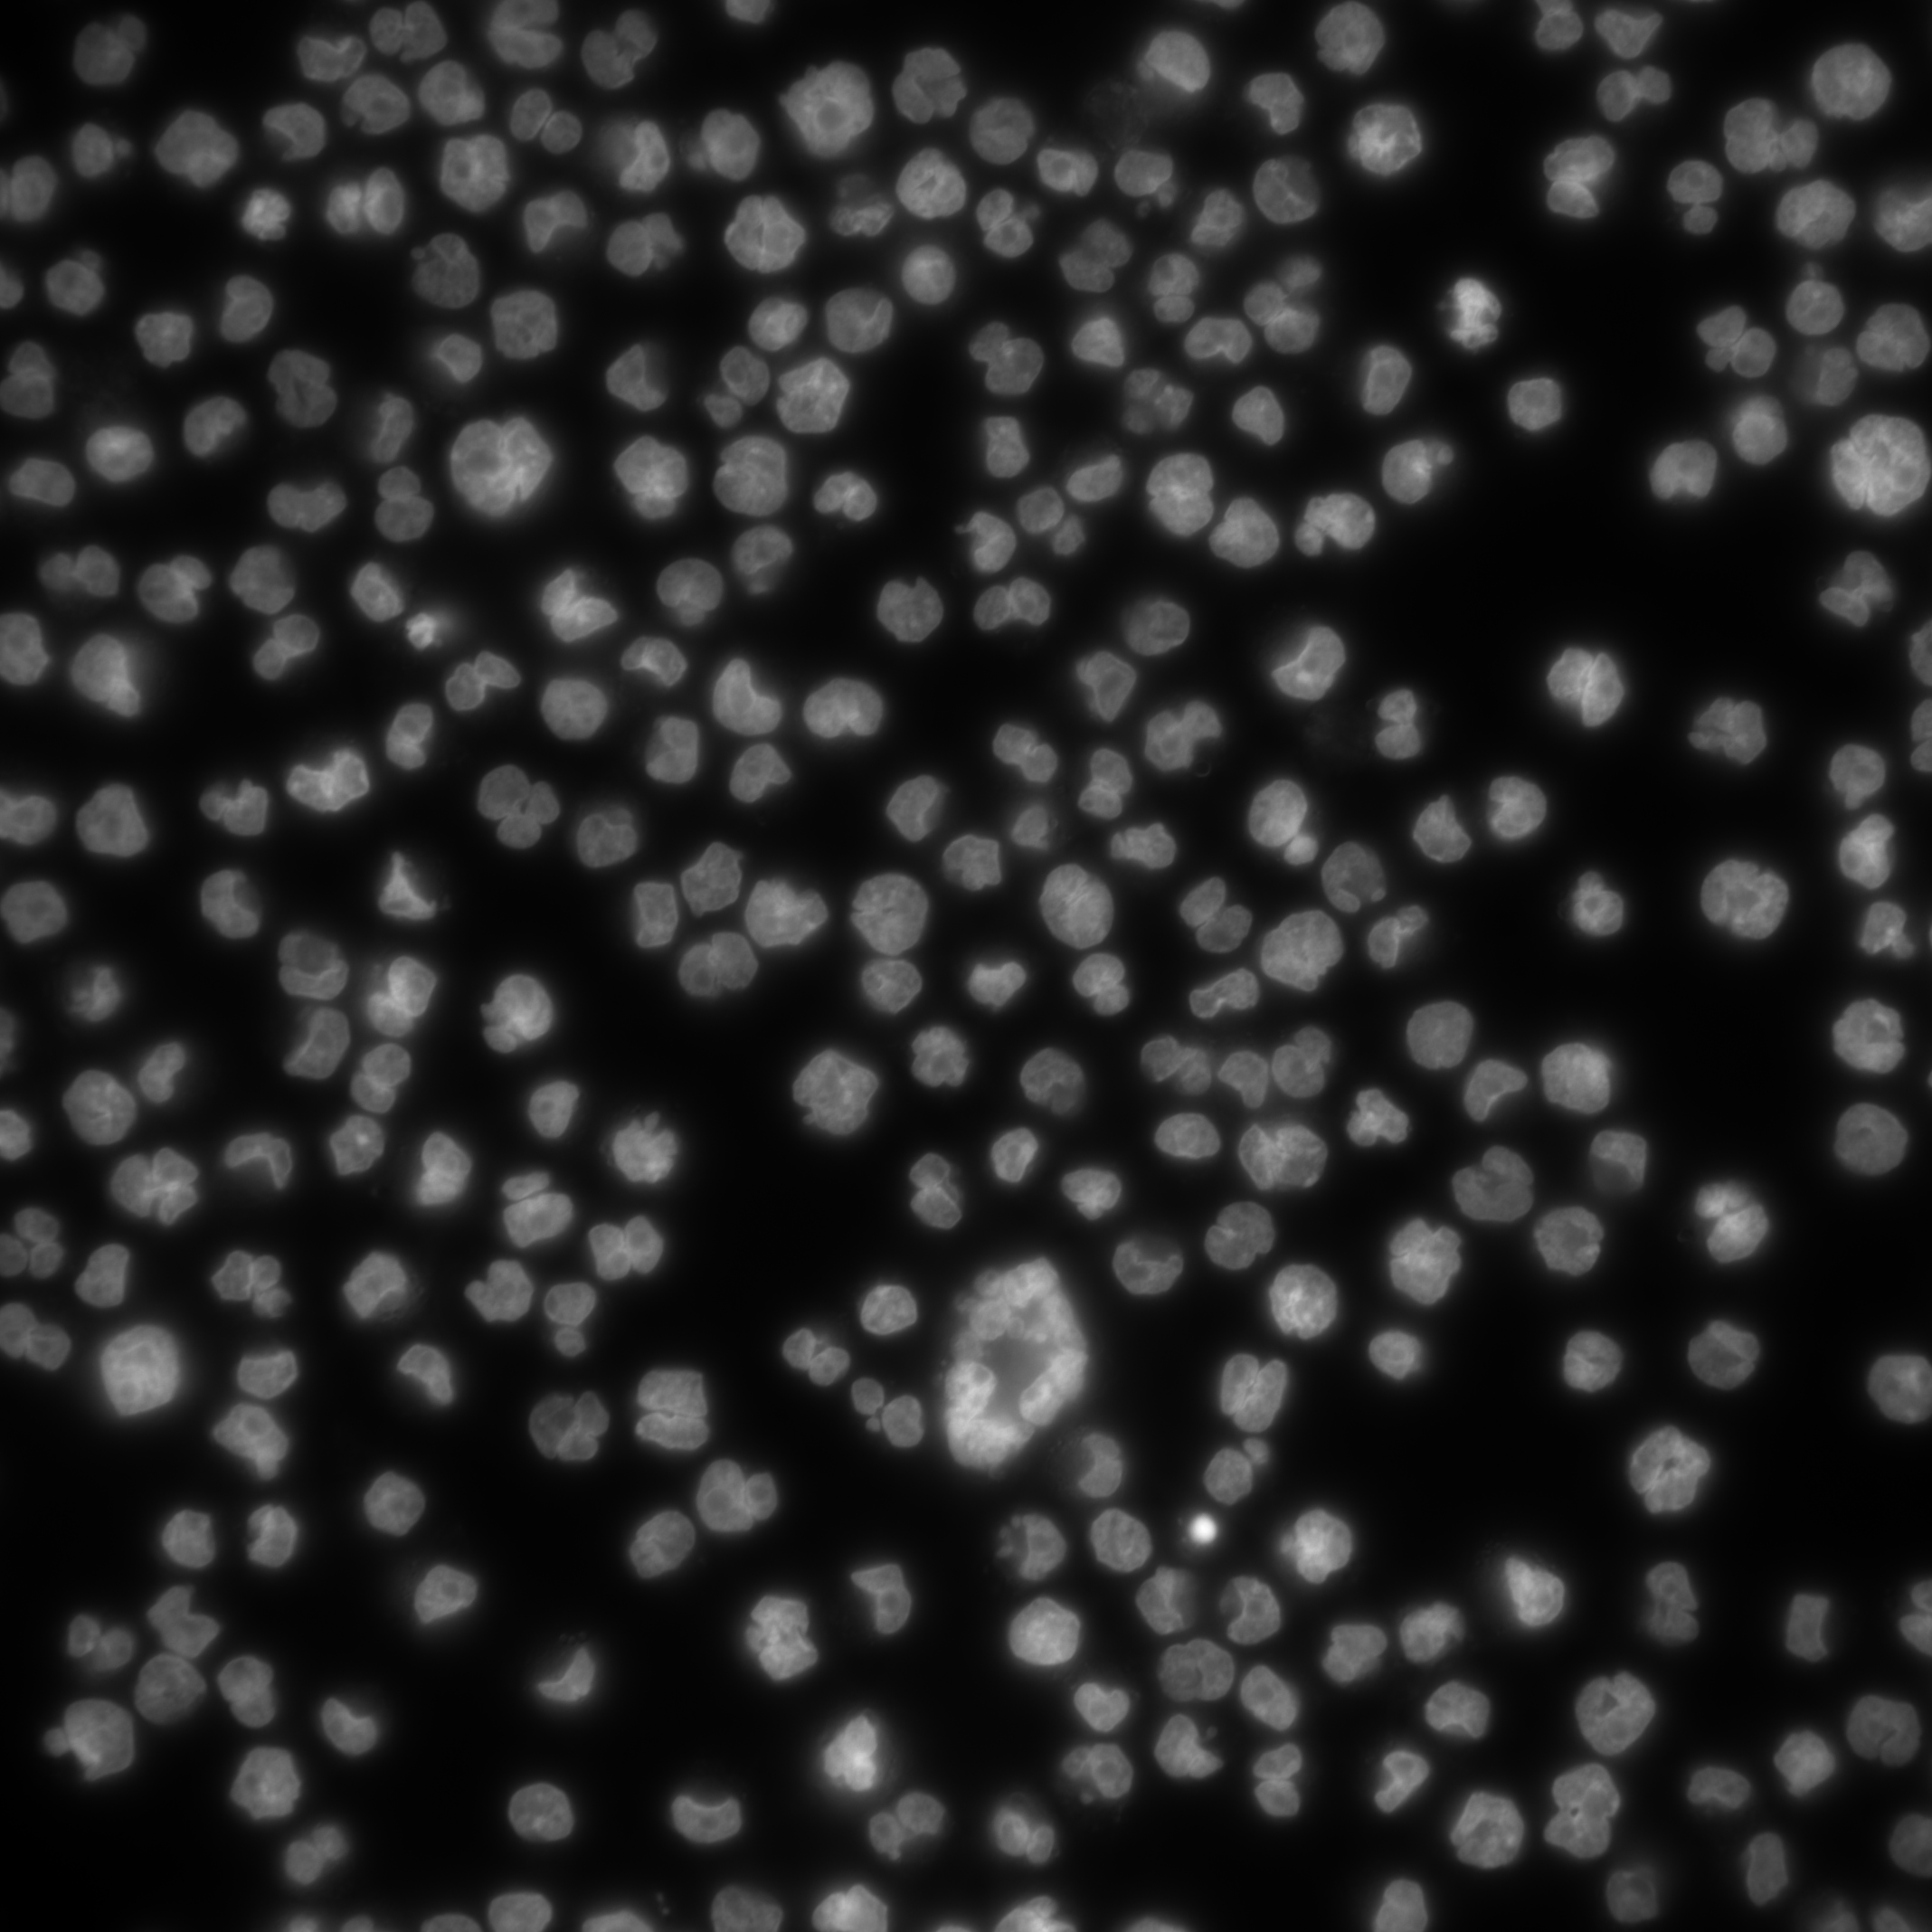
\includegraphics{bilder/lightning-conditions/lightning-4.png}
        \end{tabularx}
    \caption{Different lightning conditions}
    \label{fig:lightning_conditions}
\end{figure}